
\section{Introduction}
Invertible Neural Networks (INNs) are a class of generative neural networks which have been proposed recently as alternatives to the Generative Adversarial Network (GAN) methodology. Both are useful for generative modeling of high dimensional data distributions for which many samples are available. It is typically difficult to estimate the density function of an arbitrary high dimensional distribution, and instead the GAN solves a simpler task: learning a low dimensional parametrization of an approximation of the data manifold. The method sacrifices access to a density function, in turn prohibiting parameter estimation through maximum likelihood. In exchange for this, it is simple and computationally efficient to generate approximate samples from the data distribution.

In contrast, INNs learn an invertible map between a representation space and a data space of equal dimension. These architectures are designed to have computationally tractable Jacobians so that a prior over the representation space may be pushed forward as a differentiable density function over the entire data space. In turn, INNs permit training by maximum likelihood. This method sacrifices expressiveness of the network in exchange for a tractable Jacobian and despite their clever design, INNs are still significantly more expensive than typical GANs to train and sample from.

We study INNs in the domain of image generation. One key difficulty is that the inverse map of a trained INN may be highly non-Lipschitz, so that for particular points in the representation space it is numerically impossible to compute. One solution is to clip intermediate activations so they remain small, but this introduces image artifacts like those in Figure \ref{fig:corruption}. In most generative neural networks, representation likelihood correlates to the quality of the corresponding output image, but surprisingly, we observe empirically that points near the origin are among the most difficult to sample. 
\begin{figure}
    \centering
    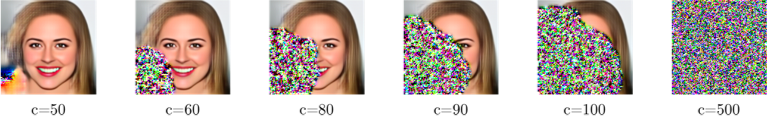
\includegraphics[width=\linewidth]{figures/figs.png}
    \caption{Corruption artifacts of a trained GLOW model when sampling the latent code $z=0$ using clipped intermediate activations. Under each image, the clipping parameter $c$ indicates the maximum allowed magnitude of any activation.}
    \label{fig:corruption}
\end{figure}

Recent work on the StyleGAN architecture highlights that large intermediate activations may be caused by unintended architectural flaws \cite{karras2019analyzing}. In light of this work, we assess the design of the GLOW architecture \cite{kingma2018glow}, a common instantiation of INNs, and pursue two main questions:
\begin{enumerate}
    \item Does the GLOW architecture have identifiable architectural oversights which cause large intermediate activations?
    \item How can the GLOW architecture be modified to reduce numerical challenges in computing the inverse map? 
\end{enumerate}

Through our experiments, we find the following:
\begin{enumerate}
    \item At a small scale, individual components of the GLOW architecture may cause large scale numerical problems while behaving as intended.  
    \item We suggest two methods to remedy this problem with minimal cost in terms of training effectiveness.
    \item We discover a hidden architectural characteristic which is necessary for stable inversion after training, motivating further investigation into the design of GLOW.
\end{enumerate}